\documentclass[tikz,border=3pt]{standalone}
\usetikzlibrary{arrows.meta,decorations.markings}
\begin{document}
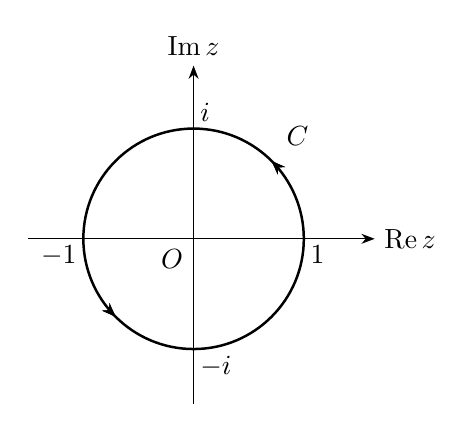
\begin{tikzpicture}[scale=1.0,>=Stealth,line width=0.9pt,
  mid/.style={postaction={decorate},decoration={markings,mark=at position #1 with {\arrow{Stealth[length=5pt]}}}}]
  % 座標軸
  \draw[line width=0.4pt,->] (-2.1,0) -- (2.3,0) node[right] {$\mathrm{Re}\,z$};
  \draw[line width=0.4pt,->] (0,-2.1) -- (0,2.2) node[above] {$\mathrm{Im}\,z$};
  \node[below left] at (0,0) {$O$};

  % 単位円 C（反時計回り）
  \draw[mid=0.125,mid=0.625] (0,0) circle (1.4);

  % 目盛り 1, -1, i, -i
  \node[below right,inner sep=2pt] at (1.4,0) {$1$};
  \node[below left,inner sep=2pt] at (-1.4,0) {$-1$};
  \node[above right,inner sep=2pt] at (0,1.4) {$i$};
  \node[below right,inner sep=2pt] at (0,-1.4) {$-i$};
  \node[above right] at (1.05,1.05) {$C$};
\end{tikzpicture}
\end{document}
